\documentclass[12pt]{article}
\usepackage[letterpaper, margin=1in, headheight=105pt]{geometry}
\usepackage{graphicx}
\usepackage{xcolor}
\usepackage{minted}
\definecolor{bg}{HTML}{282828}
\usemintedstyle{monokai}
\pagestyle{empty}

\begin{document}
\setcounter{section}{1}
\section{Homework Coding Part}
\setcounter{subsection}{1}
\subsection{Bayesian Spam Filtering}
The test error for Bayesian classifier is 11.00\%, while the majority class predictor has test error 38.56\%.
So we con conclude that the Bayesian classifier is working.
\inputminted[linenos,bgcolor=bg]{octave}{./hw2/problem2/Bayesian_spam_filtering.m}
\setcounter{subsection}{3}
\subsection{Handwritten digit classification with logistic regression}
The test error is 5.40\%.
My termination criterion is
\[ \frac{||\theta_{t+1}-\theta_{t}||}{||\theta_t||}<0.001 \]
The value of the objective function at the optimum is \(6381.5\).
Since the logistic regression rely on \(\eta(x)\) which is a probability, we take the difference between these probabilities and the threshold \(\frac{1}{2}\), and take the absolute value.
\[ \left|\eta(x)-\frac{1}{2}\right| \]
The larger this value is, the more confident the regression classifier is about its prediction.
\inputminted[linenos,bgcolor=bg]{octave}{./hw2/problem4/Handwritten_digit_classification.m}
\begin{figure}
    \centering
    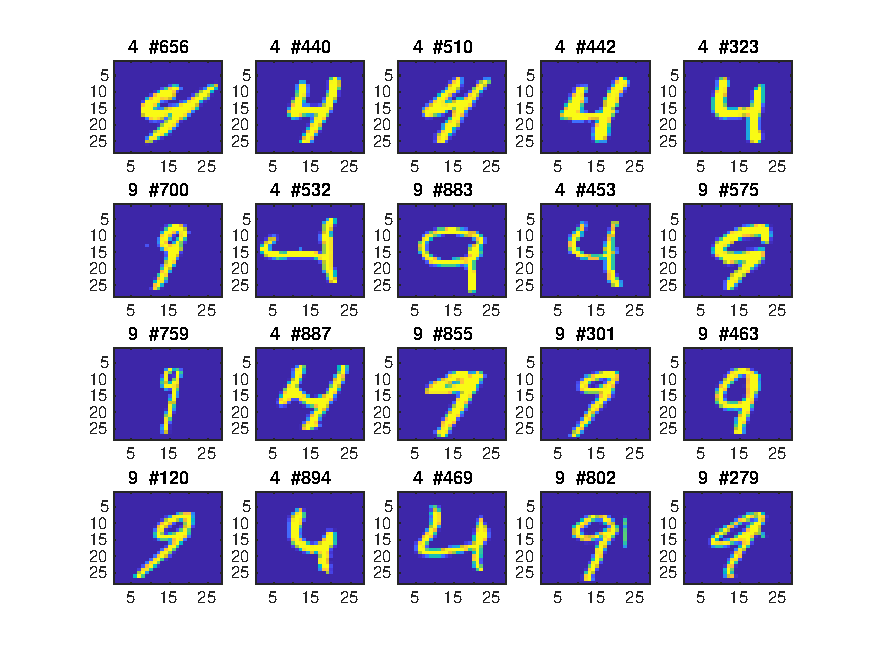
\includegraphics{./hw2/problem4/hw2p4b.pdf}
    \caption{Top 20 mis-classified images}
\end{figure}
\end{document}